\documentclass[10.5pt
%,draft
]{article}


\usepackage{ctex}
\usepackage{graphicx}
\usepackage{amsmath}
\usepackage{xcolor}
\usepackage{physics}
\usepackage{hyperref}
\hypersetup{
    colorlinks=true,
    linkcolor=Blue4Link,
    filecolor=magenta,      
    urlcolor=cyan,
    pdfauthor=徐均益
    }
\definecolor{Blue4Link}{RGB}{46,49,146}
\definecolor{myOrange}{RGB}{178,76,0}
\definecolor{green4eye}{RGB}{0,120,2}%
\definecolor{blue4eye}{RGB}{1,126,218}%
\definecolor{cyan4eye}{RGB}{31,186,190}%
\definecolor{myhighlight}{RGB}{255,214,161}
\definecolor{mybackground}{RGB}{204,232,207}
\usepackage{geometry}
\usepackage{natbib}
\usepackage{subcaption}
\usepackage{epstopdf}
\usepackage{tikz}
\usepackage{psfrag}
\usepackage{natbib}

\def\due{2023 年 5 月 26 日周五 08:40}
\def\Term{2023 年春季}
\def\Course{磁流体力学的数值模拟方法}

\renewcommand{\refname}{参考文献}
\renewcommand{\figurename}{图}
\renewcommand{\abstractname}{摘要}

\title{一维磁流体力学激波 --- 第 4 次作业\footnote{\Term\Course}}

\author{徐均益\footnote{ID: SA22214015 Email: jyxu@mail.ustc.edu.cn}
  \and
  余航\footnote{ID: SA22168021 Email: yh131996@mail.ustc.edu.cn}
  \and
  陈宇韬\footnote{ID: SA22214014 Email: chenyut@mail.ustc.edu.cn}
}

\date{%
\scriptsize%
%CAS Key Laboratory for Basic Plasma Physics, School of Earth and Space Sciences,
%\\
%University of Science and Technology of China, Hefei, Anhui 230026, China
中国科学技术大学核科学技术学院, 合肥 230026 \\
中国科学技术大学物质科学研究院等离子所, 合肥 230026
%
}

\begin{document}

\maketitle

\begin{abstract}
研究讨论一维磁流体力学 (MHD, Magnetohydrodynamics) 激波问题的有限差分数值解法, 主要采用守恒形式的\textit{Lax-Wendroff}格式,结合理论分析讨论磁声波的特性,
以及分析数值格式的计算效果。以及其他格式如隐格式和迭代法的相关尝试。
\end{abstract}

\section{引言}
磁流体力学 (MHD, Magnetohydrodynamics) 是磁流体的宏观描述,MHD方程将流体力学,麦克斯韦方程以及洛仑兹力结合起来,是一个多元非线性方程。其对应的MHD模拟是太阳物理里面非常常用的手段,比如磁绳爆发模拟等等。在本次作业中,我们在上次一维气体激波管问题的基础上,添加磁流体力学方程组,对一维磁流体力学激波问题进行模拟和分析。

\section{理论介绍}\label{DLess}
本次我们采用无量纲数值的守恒形式, 将磁流体力学方程表示为
\begin{align}
\frac{\partial U}{\partial t} + \frac{\partial F}{\partial x} = 0 \label{Eqn:MHD}
\end{align}
其中
\begin{align}
U = & \left[ \begin{array}{l}
\rho\\
\rho v^2 + H_y^2 + H_z^2 + \frac{\beta p}{\gamma -1}
\\
\rho v_x\\
\rho v_y\\
\rho v_z\\
H_y\\
H_z
\end{array} \right]\label{Eqn:Flux_U}, \\
F = & \left[ \begin{array}{l}
\rho v_x\\
\rho v_x \left(v^2 + \frac{\gamma}{\gamma - 1} \frac{\beta p}{\rho} \right) + 2(H_y^2 v_x + H_z^2 v_x - H_x H_y v_y - H_x H_z v_z)
\\
\rho v_x^2 + \frac{\beta}{2} p + \frac{1}{2} (H_y^2 + H_z^2)\\
\rho v_x v_y - H_x H_y\\
\rho v_x v_z - H_x H_z\\
v_x H_y - v_y H_x\\
v_x H_z - v_z H_x
\end{array} \right] \label{Eqn:Flux}
\end{align}
这里 $v^2 = v_x^2 + v_y^2 + v_z^2$. 若取 $\rho_0 = 1$, $p_0 = 1$, $v_0 = 1$, $H_0 = 1/\sqrt{4\pi}$, 则 $\beta = 2$.

\section{数值格式介绍}
本次实验我们尝试设计多种格式,但是经调试,只有\textit{Lax-Wendroff}格式可以维持住慢激波的形状,其他格式以及快激波等都没能完全实现。
\subsection{\textit{Lax-Wendroff}格式}
\textit{Lax-Wendroff}格式适用于守恒型方程
\begin{align}
\frac{\partial \vb w}{\partial t} + \frac{\partial \vb F}{\partial x} = 0
\end{align}
其中差分格式为
\begin{align}
u_j^{n+1} =& u_j^n - \frac{\Delta t}{2\Delta x} (F_{j+1}^n - F_{j-1}^n) \nonumber\\
& + \frac{\Delta t^2}{2\Delta x^2} \left[A_{j+1/2}^n (F_{j+1}^n-F_j^n) - A_{j-1/2}^n (F_j^n -
F_{j-1}^n)\right]
\end{align}
其中 $A = \frac{\partial F}{\partial u}$, $A$ 的表达式为
\begin{equation}
   \mqty[
0  &  0  &  1  &  0  &  0  &  0  &  0 \\
% (2 H_x \rho (H_y m_y+H_z m_z)+m_x (\rho (-\gamma E +(\gamma-2) H_y^2+(\gamma-2) H_z^2)+2 (\gamma-1) m_y^2+2 (\gamma-1) m_z^2)+2 (\gamma-1) m_x^3)/\rho^3  &  (\gamma m_x)/\rho  &  -((-\gamma E \rho+(\gamma-2) H_y^2 \rho+(\gamma-2) H_z^2 \rho+3 (\gamma-1) m_x^2+(\gamma-1) m_y^2+(\gamma-1) m_z^2)/\rho^2)  &  -((2 (H_x H_y \rho+(\gamma-1) m_x m_y))/\rho^2)  &  -((2 (H_x H_z \rho+(\gamma-1) m_x m_z))/\rho^2)  &  -((2 (H_x m_y+(\gamma-2) H_y m_x))/\rho)  &  -((2 (H_x m_z+(\gamma-2) H_z m_x))/\rho) \\
\dots  &  \dots  &  \dots  &  \dots  &  \dots  &  \dots  &  \dots \\
\frac{(\gamma-1) v^2-2v_x^2}{2 }  &  \frac{\gamma-1}{2}  &  (3-\gamma) v_x  & (1-\gamma) v_y  &  (1-\gamma) v_z  &  (2-\gamma) H_y  &  (2-\gamma) H_z \\
-v_x v_y  &  0  &  v_y  &  v_x  &  0  &  -H_x  &  0 \\
-v_x v_z  &  0  &  v_z  &  0  &  v_x  &  0  &  -H_x \\
\frac{H_x v_y-H_y v_x}{\rho}  &  0  &  \frac{H_y}{\rho}  &  -\frac{H_x}{\rho}  &  0  &  v_x  &  0 \\
H_x v_z-H_z v_x  &  0  &  \frac{H_z}{\rho}  &  0  &  -\frac{H_x}{\rho}  &  0  &  v_x ]
\end{equation}
矩阵第二行7个元素分别为
\begin{subequations}
	\begin{gather}
% (2 H_x \rho (H_y m_y+H_z m_z)+m_x (\rho (-\gamma E +(\gamma-2) H_y^2+(\gamma-2) H_z^2)+2 (\gamma-1) m_y^2+2 (\gamma-1) m_z^2)+2 (\gamma-1) m_x^3)/\rho^3   \\
-\frac{2 (H_y^2+H_z^2) v_x (1- \gamma) -2 H_x (H_y v_y+H_z v_z )(1 - \gamma) - p v_x \beta \gamma + v_x v^2 (2 - 3 \gamma + \gamma^2) \rho}{(1 - \gamma) \rho}\\
  \gamma v_x   \\
  -((-\gamma E \rho+(\gamma-2) H_y^2 \rho+(\gamma-2) H_z^2 \rho+3 (\gamma-1) m_x^2+(\gamma-1) m_y^2+(\gamma-1) m_z^2)/\rho^2)   \\
  -((2 (H_x H_y \rho+(\gamma-1) m_x m_y))/\rho^2)   \\
  -((2 (H_x H_z \rho+(\gamma-1) m_x m_z))/\rho^2)   \\
  -((2 (H_x m_y+(\gamma-2) H_y m_x))/\rho)   \\
  -((2 (H_x m_z+(\gamma-2) H_z m_x))/\rho) 
\end{gather}
\end{subequations}
其中
$ m_x = \rho v_x,
m_y = \rho v_y,
m_z = \rho v_z.$
单元边界上的值可以取
\begin{align}
A_{j \pm 1/2}^n = A(u_{j \pm 1/2}^n), \qquad u_{j \pm 1/2}^n = \frac{1}{2} (u_j^n + u_{j \pm 1}^n)
\end{align}
\subsection{数值实验设计}

考虑下列初值问题
\begin{align}
U(x,t)|_{t=0} = \left\{ \begin{array}{ll}
U_L, & \quad x < x_0 \\
U_R, & \quad x > x_0
\end{array} \right.
\end{align}
或者
\begin{align}
W(x,t)|_{t=0} = \left\{ \begin{array}{ll}
W_L, & \quad x < x_0 \\
W_R, & \quad x > x_0
\end{array} \right.
\end{align}
的有限差分数值计算. 这里 $U$ 的表达式由方程~(\ref{Eqn:Flux_U}) 给出, 具体实验时需要将$W$转化成$U$,然后再代入数值程序中进行计算。
\begin{align}
W = \left[ \begin{array}{ccccccc}
\rho,
p,
v_x,
v_y,
v_z,
H_y,
H_z
\end{array} \right]^T.
\end{align}
上标 $T$ 表示转置操作. 取 $\gamma=5/3$, $\mu=1$, $H_x=5$. 分别就如下初值条件设计实验

\subsubsection{较弱的快激波}
取 $x_0 = 0.0$, 快激波条件为
\begin{align}
W_L &= \left[\begin{array}{cccccc}
2.121,
4.981,
-13.27,
-0.163,
-0.6521,
2.572,
10.29
\end{array}\right]^T,
\nonumber\\
W_R &= \left[\begin{array}{ccccccc}
1,
1,
-15.3,
0,
0,
1,
4
\end{array}\right]^T. \label{Eqn:WFast}
\end{align}

\subsubsection{较弱的慢激波}
取 $x_0 = 0.0$, 慢激波条件为
\begin{align}
W_L &= \left[\begin{array}{ccccccc}
2.219,
0.4442,
0.5048,
0.0961,
0.0961,
1,
1
\end{array}\right]^T,
\nonumber\\
W_R &= \left[\begin{array}{ccccccc}
1,
0.1,
-0.9225,
0,
0,
1,
1
\end{array}\right]^T.\label{Eqn:WSlow}
\end{align}

\subsubsection{一维 MHD 快激波}
取 $x_0 = 0.2$, 快磁声激波的初值条件为\footnote{
  根据附件 Excel 表计算得到, 和文献 \citet{Dai1994} 稍有出入.
}
\begin{align}
W_L &= \left[\begin{array}{cccccc}
3.896,
305.9,
0,
-0.058,
-0.226,
3.951,
15.8
\end{array}\right]^T,
\nonumber\\
W_R &= \left[\begin{array}{ccccccc}
1,
1,
-15.3,
0,
0,
1,
4
\end{array}\right]^T.\label{Eqn:Fast}
\end{align}

\subsection{一维 MHD 慢激波}
同样取 $x_0 = 0.2$, 慢磁声激波的初值条件为
\begin{align}
W_L &= \left[\begin{array}{ccccccc}
3.108,
1.4336,
0,
0.2633,
0.2633,
0.1,
0.1
\end{array}\right]^T,
\nonumber\\
W_R &= \left[\begin{array}{ccccccc}
1,
0.1,
-0.9225,
0,
0,
1,
1
\end{array}\right]^T.\label{Eqn:Slow}
\end{align}

\section{实验结果及分析}
这里填入实验的图片和分析内容

\begin{figure}[htpb]
	\centering
	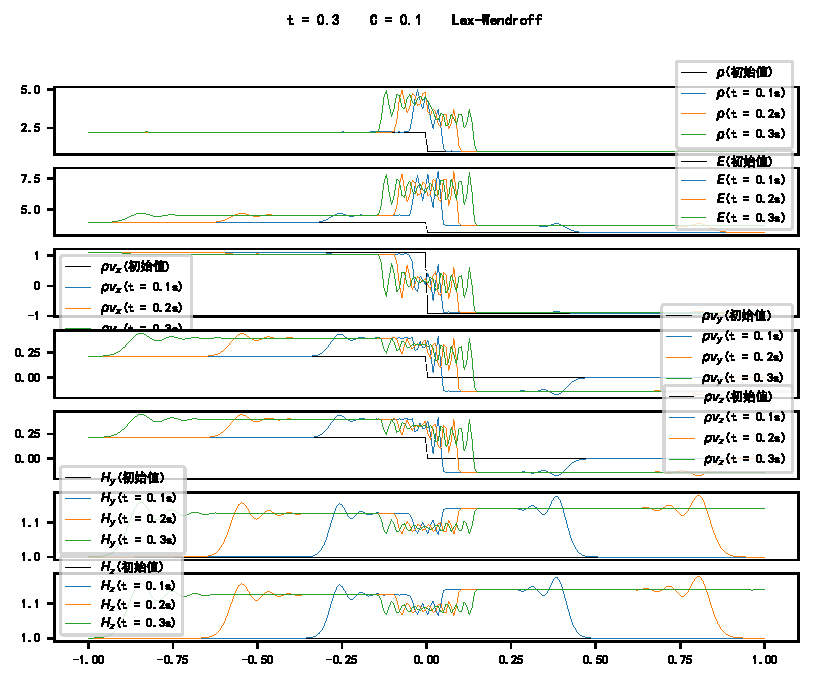
\includegraphics{figures/init2.pdf}
	\caption{较弱的慢激波。取 \(x_0 = 0.0,\) 使用 Lax-Wendroff 格式。}%
\end{figure}

\begin{figure}[htpb]
	\centering
	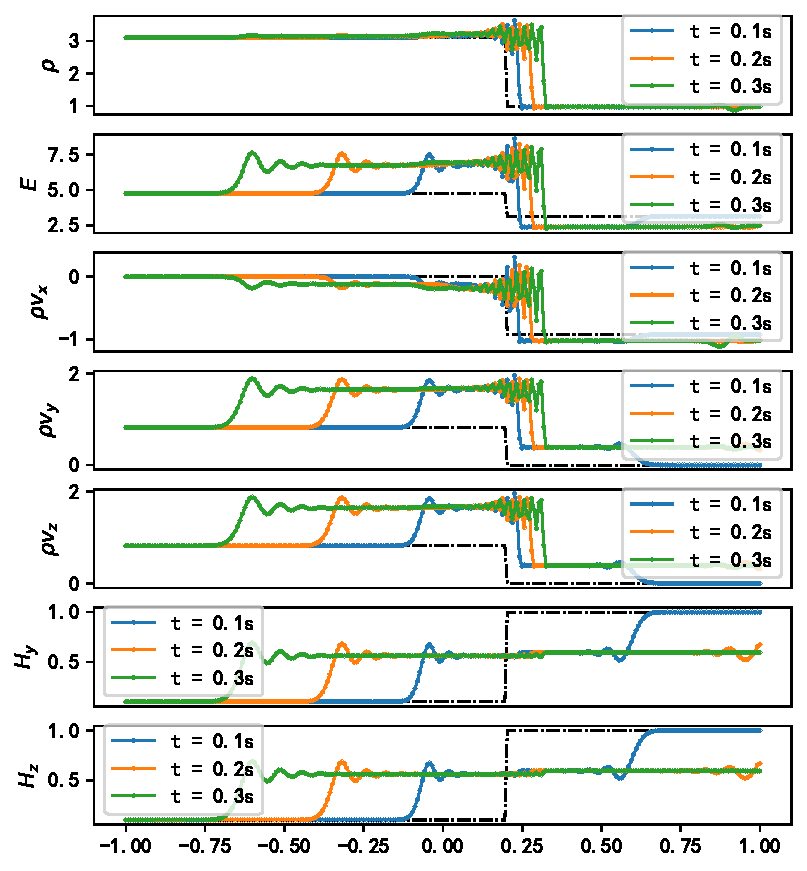
\includegraphics{figures/init4.pdf}
	\caption{一维 MHD 慢激波.取 \(x_0 = 0.2,\) 使用 Lax-Wendroff 格式。}%
\end{figure}

\section{其他数值方法尝试与分析}
这里填入其他数值方法的尝试和分析,如果周四前还填不了就把这一节给删掉

\section{附件}
\begin{enumerate}
\item
assign4.tex--本报告 \LaTeX 源文件
\item
assign4.pdf--本报告 PDF (Portable Document Format) 输出文件
\item
References.bib -- 文献文件
\item
WFast077.eps--初值条件 (\ref{Eqn:WFast}) 情况下的快激波数值结果 (TVD 格式), 133网格, 对应图~\ref{Fig:WFast} (a)
\item
WFast261.eps--初值条件 (\ref{Eqn:WFast}) 情况下的快激波数值结果 (TVD 格式), 261网格, 对应图~\ref{Fig:WFast} (b)
\item
FShockNum.eps--初值条件 (\ref{Eqn:Fast}) 情况下 (快磁声激波) 数值计算得到的物理量各时刻图形 (TVD 格式), 对应图~\ref{Fig:Fast}
\item
SShockNum.eps--初值条件 (\ref{Eqn:Slow}) 情况下 (慢磁声激波) 数值计算得到的物理量各时刻图形 (TVD 格式), 对应图~\ref{Fig:Slow}
\item
MHDShock.xlsx -- 快慢激波两侧态分析的 EXCEL 表格文件
\end{enumerate}

% 以下两行是中文文献国家标准的格式, 如果安装了这两个格式, 建议使用它们
\bibliographystyle{gbt7714-author-year}
% \bibliographystyle{gbt7714-numerical}
%

\bibliography{References}

\end{document}
